%(BEGIN_QUESTION)
% Copyright 2006, Tony R. Kuphaldt, released under the Creative Commons Attribution License (v 1.0)
% This means you may do almost anything with this work of mine, so long as you give me proper credit

En dobbeltvirkende hydraulikksylinder har 500 PSI på siden uten stempelstang og 750 PSI på stangsiden. Beregn resulterende kraft på stempelet og overført kraft i stangen, og bestem kraftretningen. Stempelet har diameter 5 tommer, og stangen har diameter 1 tomme.

$$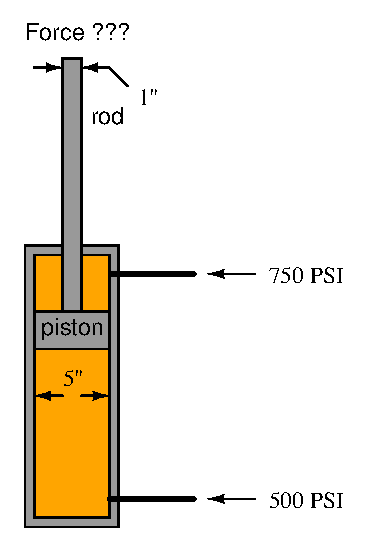
\includegraphics[width=15.5cm]{i00156x01.eps}$$

\vskip 20pt \vbox{\hrule \hbox{\strut \vrule{} {\bf Forslag til sokratisk diskusjon} \vrule} \hrule}

\begin{itemize}
\item{} Identifiser hvilke grunnprinsipper i naturfag/teknologi/matematikk som brukes i hvert løsningstrinn.
\item{} Hva skjer hvis fluidtrykk påføres nederste port og {\it vakuum} påføres øverste port? Gir dette mer, mindre eller samme kraft som når samme trykk påføres nederst og øverste port er ventilert?
\item{} Vil stempelet få resulterende kraft hvis begge porter kobles sammen med samme rør og trykksettes likt? Hvorfor/hvorfor ikke?
\item{} Hvis begge porter kobles sammen og til en trykkmåler: hva viser måleren hvis stempelet trykkes nedover? Øker, synker eller forblir målingen lik? Forklar detaljert.
\end{itemize}

\underbar{file i00156}
%(END_QUESTION)





%(BEGIN_ANSWER)

Netto kraft = {\bf 4,319.69 pund}, i nedoverretning.

\vskip 10pt

Hvis du fikk 4,908.7 pund, har du gjort en vanlig feil. Når du finner denne feilen, prøv å se hvordan oppgaven måtte vært endret for faktisk å gi 4,908.7 pund ved trykkene 750 PSI og 500 PSI.

%(END_ANSWER)





%(BEGIN_NOTES)

I dette tilfellet virker to trykk mot hverandre: 750 PSI presser nedover, mens 500 PSI presser oppover. Kraftberegningen kompliseres av at trykkene ikke virker på like arealer. Øvre trykk virker på et mindre areal fordi stangen «skygger» en del av øvre stempelflate fra 750 PSI-trykket.

\vskip 10pt

Areal av stempelbunn:

$$A = \pi r^2 = \pi \left(5 \hbox{ in} \over 2 \right)^2 = 19.635 \hbox{ in}^2$$

Effektivt areal av stempeltopp:

$$A = \pi r_1^2 - \pi r_2^2 = \pi \left(5 \hbox{ in} \over 2 \right)^2 - \pi \left(1 \hbox{ in} \over 2 \right)^2 = 19.635 \hbox{ in}^2 - 0.7854 \hbox{ in}^2 = 18.850 \hbox{ in}^2$$

\vskip 30pt

Kraft opp:

$$F = PA = (500 \hbox{ PSI}) (19.635 \hbox{ in}^2) = 9817.47 \hbox{ lb (opp)}$$

\vskip 10pt

Kraft ned:

$$F = PA = (750 \hbox{ PSI}) (18.850 \hbox{ in}^2) = 14137.17 \hbox{ lb (ned)}$$

\vskip 10pt

Resulterende kraft:

$$14137.17 \hbox{ lb} - 9817.47 \hbox{ lb} = 4319.69 \hbox{ lb (ned)}$$

%INDEX% Physics, fluids: pressure, force, and area

%(END_NOTES)
